\section{Aufbau}
\label{sec:Aufbau}

\begin{figure}[H]
         \centering
         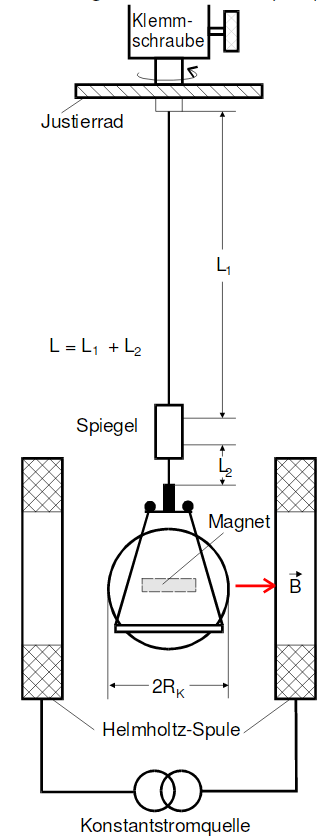
\includegraphics[width=\linewidth-150pt,height=\textheight-150pt,keepaspectratio]{content/Bilder/Aufbau.png}
         \caption{Messapperatur zur Bestimmung des Schubmoduls $G$ und des magnetischen Moments $m$ \cite{V102}.}
         \label{fig:Aufbau}
       \end{figure}

       Die Messapperatur zur Bestimmung von $G$ und $m$ setzt wie bereits in der
        Theorie erläutert auf Drehschwingungen, welche durch das Trägheitsmoment
        eines Gewichtes verursacht werden. Zur besseren Betrachtung des Drehwinkels
          $\varphi$ wird ein Spiegel verwendet. Ein Draht des zu betrachtenden
           Materials wird oben mit einer Klemmschraube fixiert. Mithilfe eines
           Justierrades lässt er sich dann nurnoch drehen. Zur Besseren
            Betrachtung wird nach einer Länge $L_1$ ein Spiegel eingesetzt. Der
             Spiegel wird über ein weiteres, kürzeres Stück Draht der Länge $L_2$ mit
             der Haltekonstruktion verbunden, in welcher sich die bereits
              beschriebene Kugel befindet.
               Um die auftretende Schwingung zu dämpfen ist ein Dämpfkonstruktion
                unter der Kugelhalterung angebracht. Zur Vereinfachung der späteren Messung von $m$ ist ein Stabmagnet
               bereits in der Kugel integriert sowie ein Helmholtzspulenpaar um die Kugel aufgestellt. Dieses wird
                 mit einer Konstantstromquelle betrieben.

                 Nun zur genaueren Betrachtung der Zeitmessung mithilfe des Drehspiegels:

                 \begin{figure}[H]
                          \centering
                          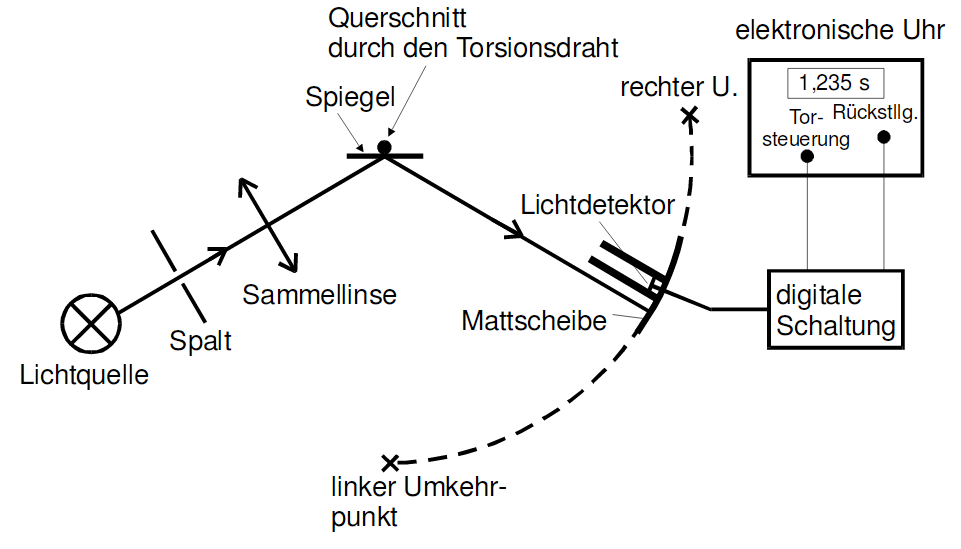
\includegraphics[width=\linewidth-150pt,height=\textheight-150pt,keepaspectratio]{content/Bilder/Drehspiegel.png}
                          \caption{Aufbau zur genauen Bestimmung der Periodendauer mithilfe eines Drehspiegels \cite{V102}.}
                          \label{fig:Drehspiegel}
                        \end{figure}

Zur besseren Betrachtung des Drehwinkels $\varphi$ wird das Licht einer Glühbirne
 mithilfe eines Spaltes und einer Sammellinse fokussiert und so ausgerichtet,
  dass es auf den Drehspiegel trifft. Während $\varphi$ sich ändert fährt der
   Lichtstrahl einen Pfad mit zwei Umkehrpunkten ab. Auf diesem Pfad ist ein
    Lichtdetektor montiert, welcher ein signal abgibt, wenn der Lichtstrahl
     ihn trifft. Die Impulse werden über eine digitale Schaltung verarbeitet und
      gelangen zu einer elektronischen Uhr, welche schließlich die Periodendauer $T$ misst.

      Die digitale Schaltung ist wie folgt aufgebaut:
